\documentclass{article}

% if you need to pass options to natbib, use, e.g.:
\PassOptionsToPackage{numbers, square}{natbib}
% before loading neurips_2019

% ready for submission
% \usepackage{neurips_2019}

% to compile a preprint version, e.g., for submission to arXiv, add add the
% [preprint] option:
%     \usepackage[preprint]{neurips_2019}

% to compile a camera-ready version, add the [final] option, e.g.:
\usepackage[final]{neurips_2019}

% to avoid loading the natbib package, add option nonatbib:
%     \usepackage[nonatbib]{neurips_2019}

\usepackage[utf8]{inputenc} % allow utf-8 input
\usepackage[T1]{fontenc}    % use 8-bit T1 fonts
\usepackage{hyperref}       % hyperlinks
\usepackage{url}            % simple URL typesetting
\usepackage{booktabs}       % professional-quality tables
\usepackage{amsfonts}       % blackboard math symbols
\usepackage{nicefrac}       % compact symbols for 1/2, etc.
\usepackage{microtype}      % microtypography
\usepackage[english]{babel}
\usepackage{graphicx}
\usepackage{wrapfig}
\usepackage{amsmath}
\usepackage{bm}
\usepackage{subfig}
\usepackage{subcaption}
\usepackage{multirow}
\usepackage[title]{appendix}
\newcommand\tab[1][1cm]{\hspace*{#1}}
\usepackage{color}
\definecolor{light}{rgb}{0.5, 0.5, 0.5}
\def\light#1{{\color{light}#1}}


\title{SVM Approaches to Cuisine Classification using Recipe Ingredients}

\author{%
  Nicholas Quek \\
  St Edmund's College\\
  University of Cambridge\\
  \texttt{nq212@cam.ac.uk} \\
}

\begin{document}
\maketitle

\begin{abstract}

In this paper, we aim to investigate the relationship between a recipe's ingredients and its cuisine type. We have tackled this as a cuisine classification task using multi-class variants of Support Vector Machines (SVMs). In addition, we explored various areas for optimisation to improve the classifier performance. 

\end{abstract}

\section{Introduction}

% Why cuisine type vs ingredient is important
Leveraging on the power of social media, many recipe sharing services such as Yummly \cite{yummly} have sprung out over the years. These serve a wide variety of functions from sharing a personal recipe with friends to creating recipes for leftover ingredients, the most popular of which is recipe recommendation. It comes to no surprise that much effort has been devoted to optimising the recommendations. The type of cuisine is often a primary consideration when deciding on what to eat, a crucial piece of information for any recommendation service.

% Impact of paper
Discovering connections between cuisine type and ingredients would enable food databases and recipe recommendation systems to automatically categorise new recipes by cuisine solely using the recipe ingredients. The cuisine information could also be utilised as an additional filter for recipe recommendation. Course/menu planning can use cuisine categorisation by placing recipes from the same cuisine together to build a coherent theme.

% What we do in this paper
In this paper, we use a recipe dataset made available through a Kaggle competition to perform cuisine classification. We experimented with different feature extraction techniques and multi-class SVMs variants. We achieve the best accuracy by first pre-processing the training data to eliminate textual clutter. The pre-processed data is converted to tf-idf vectors, ignoring terms which appear in fewer than 10 recipes, and then used to train a SVM One-Versus-All model with a RBF kernel. The model achieves a classification accuracy of 82.31\% after training on a dataset of 39,774 recipes. This accuracy score would place the model at 5\textsuperscript{th} place on the Kaggle public leaderboard for the competition.

\section{Related Work}
Past research has investigated the use of SVMs in on the same classification task, automatic cuisine classification from ingredients \cite{autorecipe}, but on a different dataset. The dataset used in \cite{autorecipe} was from food.com, a recipe-sharing website, while we use a dataset from Kaggle \cite{kaggle}. The main difference is that our dataset consists of a total of 20 classes, significantly more than the 5 in \cite{autorecipe}, making our task more difficult. The food.com dataset also contains recipe names, which are absent in the Kaggle one. 

Similar work on the same dataset as ours have also been done \cite{KaggleRecipe}. The authors explored a variety of classification techniques (Naive Bayes Classifier, Nearest Neighbour and SVM) and compared their performance. In this paper, we focus primarily on SVMs and investigate the performance of different multi-class flavours of SVMs.

\section{Dataset}
The dataset of recipes was obtained from “What’s cooking?”, a Kaggle competition \cite{kaggle} hosted by Yummly. Each recipe consists of a list of ingredients as well as a cuisine label. The dataset contains 39,774 labelled recipes, 2,965 unique ingredients and 20 cuisine types. The cuisine distribution is unbalanced, with the dominant cuisine, Italian, making up 19.7\% of the recipes while other cuisines such as Brazilian, Filipino, Irish and Jamaican only contribute $<$2\% each.

While the Kaggle competition have concluded, the submission functionality is still available. The organisers have put aside a test set with an additional 9,944 recipes for model evaluation. Labels for the test set is not known to the participants. We used this test set for evaluation, freeing up the entire training dataset for training purposes.

\section{Methodology}\label{methods}
Given a list of ingredients, there are multiple steps to obtain a classifier. Figure \ref{img:pipeline} shows the steps in designing said classifier. There is a multitude of methods which could be applied at each stage of the pipeline, each with their advantages and disadvantages. This paper investigates different methods at the various stages of the pipeline.  

\begin{figure}[h]
  \centering
  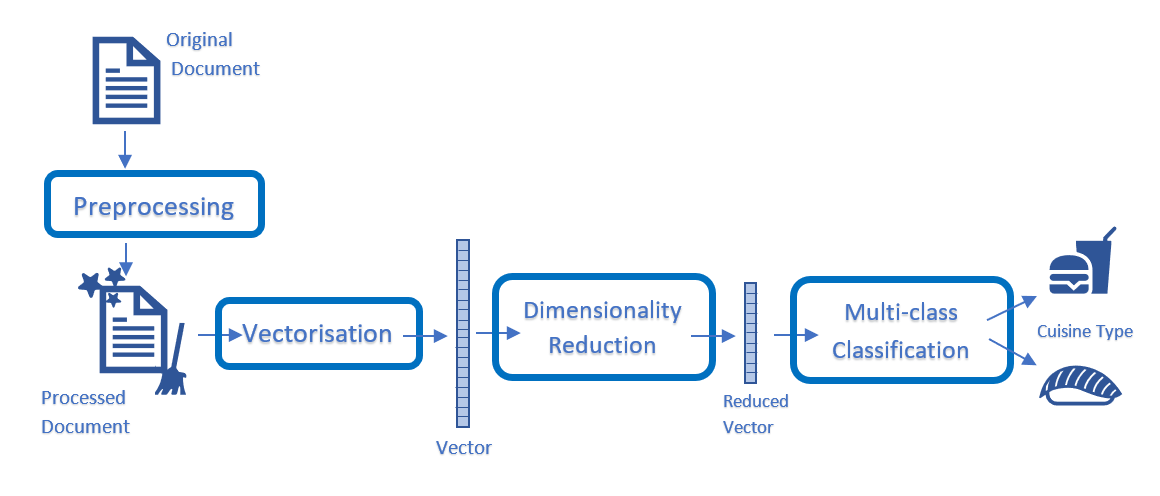
\includegraphics[width=14cm]{Flowchart.PNG}
  \caption{Pipeline for Classification Task}
  \label{img:pipeline}
\end{figure}

\subsection{Pre-processing}
Each recipe in the dataset is represented by a list of ingredients. Upon further inspection, we observed that some ingredients would be difficult to work with if we do not perform any pre-processing. Some samples of tricky ingredients are as follows:

\begin{itemize}
    \item Hidden Valley® Original Ranch® Dressing
    \item 2 1/2 to 3 lb. chicken, cut into serving pieces
    \item potatoes, potato
    \item artichok heart marin
\end{itemize}


The first ingredient contains special characters. The second has unnecessary information such as quantity and preparation details. The third shows different inflections of the same root word. The final example contains misspellings and abbreviations. We pre-processed each ingredient by first converting them into lowercase text. All numbers and punctuation are then removed. Units of measurements (e.g. kg, lb) are stripped. Accents (e.g. purée) are replaced with their ASCII projection using \light{Unidecode \cite{unidecode}}. We employed \light{NLTK \cite{nltk}} to perform lemmatisation to reduces the inflected words to an English root word.

\subsection{Vectorisation}
Once we have the processed list of ingredients, we need to convert the textual data to a format which could be handled by classification algorithms. We employed the following techniques to vectorise our recipes. The resulting vectors are then normalised by the Euclidean norm (L2 norm).

\subsubsection*{Bag-of-words}
Each recipe is represented using the bag-of-words model, which disregards syntactic information (such as grammar and word order) and captures only the term frequency, which is the number of times a term appears in the text. Each dimension of the generated vector corresponds to a unique word in the vocabulary, resulting in the output vector having a dimensionality equal to the size of the vocabulary. In our case, the vectors produced have 2,793 dimensions corresponding to the 2,793 terms. A characteristic of the generation approach is the resulting vector would be extremely sparse, with only a few non-zero values.

\subsubsection*{Term Frequency-Inverse Document Frequency (tf-idf)}
Term frequency is often not the best representation. In this dataset, common ingredients like "pepper" and "salt" appear in more than half the recipes. These common ingredients, therefore, tell us less about the recipes compared to the other ingredients. Term frequency ignore this information and assign them a weight equivalent to the number of occurrences in the recipe, failing to emphasise the more discriminative ingredients.

To address the weighting issues introduced by term frequency, we introduce an additional weighting factor, inverse document frequency ($idf$), given below. The inverse document frequency is a measure of how much information a term provides. By combining term frequency with inverse document frequency, we assign more importance to terms which occur in fewer documents. This addresses the problem of common ingredients getting similar emphasis as more discriminative ingredients.

$$ idf(t) = \log{\dfrac{1 + n}{1 + df(t)}} + 1 $$
where $n$ is the total number of recipes, and $df(t)$ is the number of recipes that contain the term $t$. 

\subsection{Dimensionality Reduction}
Both bag-of-words and tf-idf generate vectors with dimensionality equal to the number of unique words in the vocabulary (2,793 in our case). As the performance of SVMs would suffer if too many irrelevant features are included in the feature space, we investigate several dimensionality reduction techniques to eliminate noise in the dataset and verify if any of them would improve our classifiers.

\subsubsection*{Vocabulary Fine-tuning}
The dimensionality of our vectors depends on the size of the vocabulary. We can reduce the size of our vocabulary by excluding non-informative words, which tend to have either extremely high or extremely low document frequencies. For example, a term with low document frequency could be a misspelling and therefore would only occur in a small set of recipes, while a term with high document frequency might not be as informative as one that occurs only in a select subset of the data (i.e. in a particular set of cuisines). In both cases, removing these terms should improve the utility of the vector representations.

\subsubsection*{Single Value Decomposition (SVD)} 
Matrix factorisation is a common technique used to project data from a high dimensionality space to a lower dimensionality one. In SVD, a large matrix is factorised into three component matrices, $USV$. We adjust the rank of $S$ to the dimensionality of our reduced space. We then reconstruct the features of each recipe using $US$. By setting the rank of $S$ to k, we are identifying k dimensions where the information-to-noise ratio is the highest, ignoring the others. This projects the vector to a lower dimensionality space. This paper utilises the \light{scikit-learn \cite{scikit-learn} (TruncatedSVD)} implementation to perform the dimensionality reduction. 

The computational complexity of SVMs depends on the number of features. While it reduces the dimensionality, performing SVD on the sparse vectors from tf-idf increases the number of features as the vector becomes dense in the new reduced space. The result of performing SVD on this dataset is an explosion of features, increasing computation time significantly.

\subsection{Multiclass Classification}
Support Vector Machines are intrinsically a binary classifier. This paper considers two general strategies for tackling multi-class classification problems. The first strategy involves decomposition of the multi-classification problem into multiple single classification problems. For this strategy, we investigate the performance of One-versus-All (OvA) and One-versus-One (OvO) classifiers. The second strategy is to utilise a hierarchical structure to divide the output space. In this paper, a binary tree structure is used in a SVM Binary Decision Tree (SVM-BDT). The performance of Twin SVMs has been shown to be comparable to SVM (superior in some datasets) in past work \cite{TSVM}. This paper investigates if employing Twin SVMs as a substitute for a traditional SVM would result in better performance.

\subsubsection*{One-versus-All SVM (SVM OvA)}
The most popular approach to multiclass classification using SVMs is to reduce the problem of classifying among $k$ classes into $k$ binary problems, where each problem discriminates a given class from the other $k-1$ classes. The i\textsuperscript{th} classifier is trained with the recipes in the i\textsuperscript{th} class with positive labels, and all other recipes with negative labels. The prediction for a given data point is the class whose classifier assigned it as positive. In the event of a tie (e.g. more than one/none of the classifiers assigned it as positive), we classify the point according to the classification confidence levels of the underlying binary classifiers.  We used \light{scikit-learn (OneVsRestClassifier)} for this flavour of multi-class classification.

\subsubsection*{One-versus-One SVM (SVM OvO)}
Another method used to decompose the multi-class problem is the One-versus-One approach \cite{OvO}. This method constructs $\tfrac{1}{2}k(k - 1)$ classifiers where $k$ is the number of classes. Each classifier is trained only on data from the two classes it is trying to differentiate. We used a voting strategy where the data point is assigned to the class with the largest number of votes. In the event of a tie, we compute the overall confidence by summing over the pair-wise classification confidence levels of the underlying binary classifiers. We used \light{scikit-learn (OneVsOneClassifier)} for this flavour of multi-class classification.

\subsubsection*{SVM Binary Decision Tree (SVM BDT)}

\begin{wrapfigure}[19]{r}{5.5cm}
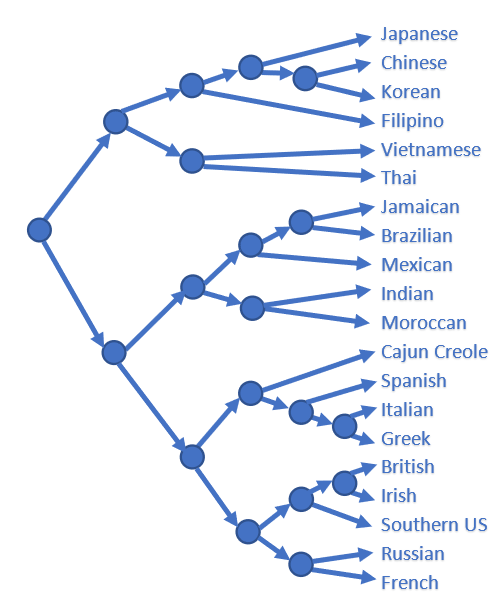
\includegraphics[width=5.5cm]{BinaryTree.PNG}
\caption{Divison of output space using KMeans Clustering}
\label{img:binarytree}
\end{wrapfigure} 
The SVM BDT \cite{BDTSVM} is a hierarchical approach to the multi-class classification problem. It employs a tree structure to perform hierarchical division of the output space. At each node, a binary classifier makes the discrimination between two different child class clusters. The process continues until the leaf nodes contain exactly one class. A total of $k-1$ classifiers are trained for a problem with $k$ classes. Only data points from the relevant class clusters are required to train the node classifier. While the root node would require the entire dataset, as we progress down the tree, the data points required decreases. This results in shorter training times compared to both OvA and OvO approaches. We relaxed the constraints on the tree such that it obtains the most natural separation rather than enforcing the classes be evenly divided at each step. 

There exist many ways to divide $k$ classes into two groups, and proper grouping is crucial for SVM-BDT to perform. Knowledge of how the classes are clustered is required to perform this division. We combined all recipes from the same class into a giant recipe and apply tf-idf to obtain a class vector. The class vectors are then mapped to the same kernel space as the classifier. K-Means clustering using \light{scikit-learn (SpectralClustering)} is then performed to identify two disjoint clusters. We apply the clustering algorithm recursively within the discovered clusters to construct the binary tree. Figure \ref{img:binarytree} shows the output space division using a RBF kernel ($\gamma=1$).

\subsubsection*{Twin SVMs}
Twin SVMs \cite{TSVM} is an alternative to traditional (max-margin) SVMs. Max-margin SVM seeks to maximise the margin between two disjoint half planes. In Twin SVMs, we generate two nonparallel planes such that each plane is closer to one of the two classes and is as far as possible from the other. Figure \ref{fig:tsvm} provides a visual representation of the differences. In terms of performance, Twin SVM have been shown to achieve comparable (if not superior) results to SVMs for certain datasets \cite{TSVM, LTSVM}. As such we deem it worthwhile to investigate if it would perform better for this classification task. We used \light{LightTwinSVM \cite{LTSVM}} for the Twin SVM implementation.

\begin{figure}%
    \centering
    \subfloat[Max Margin SVM]{{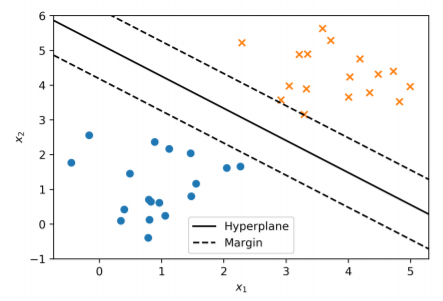
\includegraphics[width=5cm]{MaxMargin.PNG} }}%
    \qquad
    \subfloat[Twin SVM]{{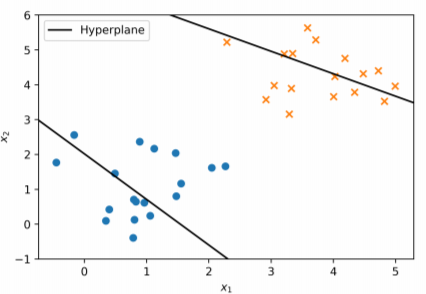
\includegraphics[width=5cm]{TwinSVM.PNG} }}%
    \caption{ Differences between Twin SVM and SVM \cite{LTSVM}}%
    \label{fig:tsvm}%
\end{figure}


\section{Experimental Results} \label{experiments}
In Section \ref{methods}, we designed a multi-stage pipeline to create the classifier. At each stage, we introduced several techniques. In this section, we compare and evaluate the various techniques, to justify our eventual model.

\subsection{Experimental Setup}
The models are trained using the entire training set. The hyperparameters of the models (namely C, the regularisation parameter for SVMs, and kernel parameters) were selected using a grid search with five-fold cross validation. The test set which contains 9944 recipes held-out by the organisers was used for the evaluation. The predictions on the test set were submitted to the Kaggle competition page to obtain a final accuracy score. 

\subsection{Performance Analysis}
\subsubsection*{Effects of pre-processing}
We utilised the \light{scikit-learn (Tokenizer)} to convert the documents into tokens for vectorisation. Before pre-processing, tokenisation resulted in a vocabulary of 3051 terms. Some of these terms in this vocabulary contained numbers and accents. Following pre-processing, the vocabulary shrinks to 2793 terms. 

Table \ref{preprocessing} shows the accuracy score provided by Kaggle upon submission of the models. Both models utilised vectors generated using tf-idf without any dimensionality reduction, followed by SVM OvA with a Radial Basis Function (RBF) kernel.


\begin{table}[h]
\centering
\begin{tabular}{|c|c|}
\hline
\textbf{Approach}& \multicolumn{1}{l|}{\textbf{Accuracy}} \\ \hline
No pre-processing & 0.81868                       \\
Pre-processing    & 0.81948                       \\
 \hline
\end{tabular}
\caption{Effects of pre-processing}
\label{preprocessing}
\end{table}

Surprisingly, the difference in performance is not significant. This could be due to several factors. The dataset only contains ingredients. Compared to traditional natural language processing datasets which contain syntactic information such as grammar, it is considerably cleaner. This would mitigate the effects of any pre-processing steps. Another possible factor would be inherent bias prevalent in both the training and test data. E.g. accents are language-specific and therefore would be more indicative of a certain cuisine. The classifier might exploit these biases to obtain better classification on the test data. Elimination of such information would negate some of the advantages of having cleaner data.  

\subsubsection*{Comparison between vectorisation methods} 
The models in Table \ref{vectorisation} utilised the pre-processed data for training. The models employed different vectorisation methods without any dimensionality reduction, followed by SVM OvA with a RBF kernel.

\begin{table}[h]
\centering
\begin{tabular}{|c|c|}
\hline
\textbf{Approach}    & \multicolumn{1}{l|}{\textbf{Accuracy}} \\ \hline
Bag-of-words & 0.81777                       \\
tf-idf       & 0.81948                       \\
 \hline
\end{tabular}
\caption{Different Vectorisation Methods}
\label{vectorisation}
\end{table}

As expected, tf-idf performed better than the bag-of-words approach which only involves term frequency. In typical NLP tasks, the performance difference between bag-of-words and tf-idf is drastic. In our case, the difference is not as significant. This is likely because term frequencies tend to be small in most recipes; ingredients often do not appear multiple times in the ingredient list. As a result, the effect of placing less weight on these common ingredients is diminished.

\subsubsection*{Effects of dimensionality reduction}
We investigated if the generated vectors contain noise which can be eliminated by dimensionality reduction. Table \ref{dimredu} shows the model performances of vocabulary fine-tuning and SVD with different output dimensions. The models reduced the dimensions of the tf-idf vectors generated on the pre-processed data. The reduced vectors are then passed to SVM OvA with a RBF kernel.

\begin{table}[h]
\centering
\begin{tabular}{|c|c|c|c|}
\hline
\textbf{Approach}                  & \textbf{Parameters}   & \textbf{Dimensions} & \textbf{Accuracy} \\ \hline
\multirow{5}{*}{Vocab Fine-Tuning} & df \textgreater{}= 2  & 2240       & 0.82119  \\ \cline{2-4} 
                                   & df \textgreater{}= 10 & 1377       & 0.82310  \\ \cline{2-4} 
                                   & df \textgreater{}= 20 & 1081       & 0.81878  \\ \cline{2-4} 
                                   & df \textless{}= 250   & 2445       & 0.44318  \\ \cline{2-4} 
                                   & df \textless{}= 100   & 2223       & 0.28740  \\ \hline
\multicolumn{2}{|c|}{\multirow{2}{*}{SVD}}                 & 2000       & 0.82180 \\ \cline{3-4} 
\multicolumn{2}{|c|}{}                                     & 1500       & 0.82210  \\ \hline
\multicolumn{2}{|c|}{No Dimensionality Reduction}          & 2793       & 0.81948  \\ \hline
\end{tabular}
\caption{Different Dimensionality Reduction Techniques}
\label{dimredu}
\end{table}

An observation we made when we varied the parameters of the vocabulary fine-tuning method is that extremely common terms are much more informative than rare terms. When we set the maximum document frequency ($df$) to 250, we eliminated the most common 248 terms. By doing so, we ignored crucial information in our dataset, resulting in poor accuracy of 44.3\%. Enforcing a stricter document frequency ceiling only served to exacerbate the decline in accuracy. On the other hand, we eliminated a total of 553 terms which occurs only once, by setting the minimum document frequency to 2. The 0.2\% improvement in accuracy indicates that these rare terms are more noisy than informative. Elevation of the document frequency floor improved accuracy to an extent before we started seeing a decrease in accuracy. The peak accuracy occurs when the floor is set to 10. It appears that a document frequency of 10 is the sweet spot where noisy terms (caused by misspellings, etc) are eliminated while cuisine-specific niche ingredients are retained.

\begin{wrapfigure}[16]{l}{6cm}
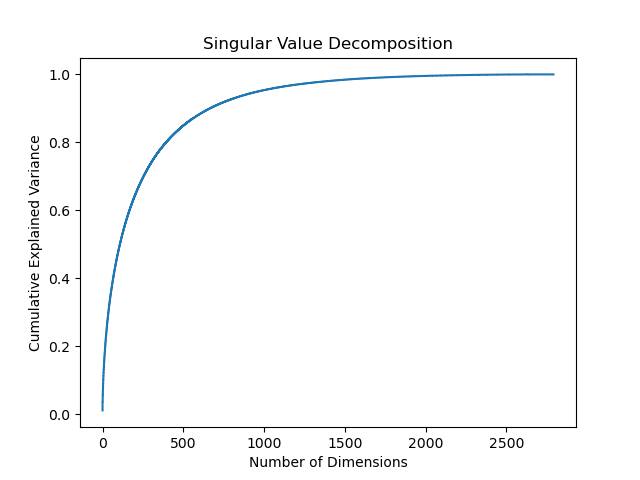
\includegraphics[width=6cm]{svd.PNG}
\caption{Explained Variance for SVD}
\label{img:svd}
\end{wrapfigure} 

Figure \ref{img:svd} shows the explained variance for the SVD approach. A dataset which is well-suited for SVD should have the curve as close to the top left-hand corner of the graph. For our dataset, the curve is far from the corner. As a result, we require a large number of dimensions in order to capture a significant portion of the variance. Therefore, it is unlikely that SVD would significantly improve our classifier.

Overall, it appears that the utility of the tf-idf vector can be improved using dimensionality reduction, achieving an accuracy improvement of 0.004. However, the performance of our baseline model (without dimensionality reduction) would have an accuracy deviation of 0.0075 at a 95\% confidence interval. Therefore, we cannot make claims about whether any of the dimensionality reduction techniques improve the performance.

\subsubsection*{Kernels Selection}
The max-margin support vector classifier essentially attempts to divide the space occupied by the data into two using a plane. Non-linearly separable data is challenging for the classifier. A common technique is to transform the data in its raw representation into a higher dimensional vector space in the hopes that the data becomes linearly separable in the higher dimensional space. SVMs uses a set of mathematical functions that are defined as the kernel to perform this data transformation. Different types of kernel functions would map the data into different vector spaces. We investigated different kernel functions to find the representation which is the most linearly separable.  

\begin{table}[h]
\centering
\begin{tabular}{|c|c|}
\hline
\textbf{Kernel}     & \textbf{Accuracy} \\ \hline
Linear     & 0.78580  \\ \hline
RBF        & 0.82310  \\ \hline
Polynomial & 0.81938  \\ \hline
Sigmoid    & 0.75261  \\ \hline
\end{tabular}
\caption{Kernel Selection}
\label{kernels}
\end{table}

Table \ref{kernels} shows the performance of different kernels. The data is pre-processed, converted to tf-idf vectors after vocabulary fine-tuning with a minimum document frequency of 10. The reduced vectors are passed to a SVM OvA classifier with the relevant kernel function. The performance of the linear kernel is acceptable. This indicates that the data in its original vector space is largely linearly separable. However, there are still portions in the space where it is difficult to linearly separate the data, as shown by the improvement when the RBF kernel is employed. For the polynomial kernel, we explored the performance of different degrees. With tuning of the other parameters, the degree of the kernel did not significantly affect the accuracy.

\subsubsection*{Comparison between multi-class classifiers}
\begin{table}[h]
\centering
\begin{tabular}{|c|c|}
\hline
\textbf{Multiclass Flavour} & \textbf{Accuracy} \\ \hline
SVM OvA            & 0.82310  \\ \hline
SVM OvO            & 0.81023  \\ \hline
SVM BDT            & 0.80128  \\ \hline
Twin SVM           & 0.77956  \\ \hline
\end{tabular}
\caption{Performance of various multi-class SVMs}
\label{multiclass}
\end{table}

Table \ref{multiclass} shows the performance of the different multi-class SVM variants. The data is pre-processed, converted to tf-idf vectors after vocabulary fine-tuning with a minimum document frequency of 10. The RBF kernel is utilised for all the variants.

From the results, SVM OvA achieves the highest accuracy. While it is tempting to conclude that this strategy is the best choice for this classification task, we need to consider that during the technique selection for earlier stages (pre-processing, vectorisation, dimensionality reduction), we opted to use the OvA approach for their evaluation. The better performance of the OvA strategy could be attributed to the earlier technique choices being optimised for the OvA strategy. The performances of the other variants might be improved if we re-tuned some parameters of the earlier stages. The significantly poorer performance of Twin SVM is likely due to incompatibility. Since the Twin SVM separation strategy differs significantly from the max-margin SVM, there is no guarantee that the vectors optimised for a max-margin SVM would work well with a Twin SVM. More investigation would be required in order to conclude that Twin SVM performs poorer compared to a max-margin SVM on this dataset.  

For SVM BDT, we observed that at each node, the binary classifier was able to separate the data into the two child class clusters with high accuracy (90 - 98\%). However, a data point must pass through a series of nodes, before it gets assigned to a single class. The process of passing through multiple nodes degrades the accuracy by a multiplicative factor. The primary advantage SVM BDT have over OvA and OvO is that the effects of individual binary classifiers are much more pronounced. Therefore, this reveals avenues for fine-grained optimisation of the binary classifiers. However, for this task, the accuracy of the binary classifiers are already extremely high (\textgreater{90\%}), leaving little room for optimisation. We hypothesise that SVM BDT would perform significantly better in classification problems with a smaller group of classes or where the classes are significantly more difficult to differentiate, allowing for fine-grained optimisation of the individual classifiers.

\section{Evaluation}
The best model we obtained from Section \ref{experiments} is a SVM OvA classifier trained on tf-idf vectors generated from pre-processed data after vocabulary fine-tuning with minimum document frequency set to 10.

Unfortunately, the test dataset used in Section \ref{experiments} would not be able to provide us with any insights since the cuisine labels are not available to us. Hence, to gain meaningful insight into the performance of our best model, we held out 10\% of the training dataset as a test dataset and re-trained a model with hyperparameters found in Section \ref{experiments} on the remaining data. Figure \ref{img:cm} shows the confusion matrix produced when the best model is evaluated on the held-out test data. Table \ref{precision} shows the precision score of the different classes. While our model classifies most cuisine types with a high degree of precision, it also performs extremely poorly for a small number of cuisines (Spanish and Russian), only achieving a precision of slightly above 50\%. An interesting observation is that Italian cuisine has a high precision of 0.90. In comparison, French cuisine only have a precision of 0.64. While these two cuisines are similar in terms of ingredients, it is likely that the class imbalance in the training set is causing the skew in predictions. The classifier is encouraged to label ambiguous French-Italian recipes as Italian due to the higher probability of a recipe being Italian. Therefore, we observed more French recipes being wrongly labelled Italian rather than Italian recipes being labelled French. 
The dataset originated from a competition where accuracy was the criterion for evaluation. Staying faithful to the competitive nature of the dataset, we emphasised accuracy over precision during the training of our classifier. This emphasises the classification bias observed. However, if we were to construct a classifier for use in the wild, we would include precision as a criterion during training to produce a classifier which does not favour a specific cuisine over others.

\section{Future Work}

In this paper, when we investigated the performance of a technique during a stage in the pipeline, the other stages were kept constant. While this approach does explore the various options available, we might end up in a local minimum. Ideally, we would like to be able to perform a grid search over techniques across all stages of the pipeline. However, the explosion in search space makes it infeasible to perform within the experimental constraints. 

In Section \ref{experiments}, the performance of the Twin SVM was not as desirable. We reasoned that it could be due to incompatibility between the features and Twin SVM model. An investigation into this hypothesis could reveal deeper insights into Twin SVM, uncovering situations where it thrives or suffers. 



\begin{minipage}{\textwidth}
\begin{minipage}[b]{0.7\textwidth}
\centering
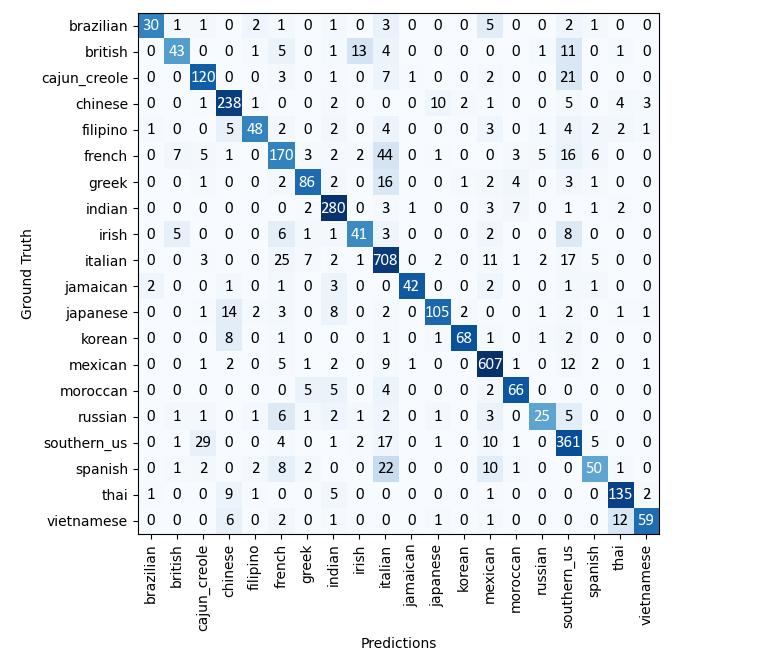
\includegraphics[width=10cm]{cm.PNG}
\captionof{figure}{Confusion Matrix}
\label{img:cm}
\end{minipage}
\hfill
\begin{minipage}[b]{0.29\textwidth}
\centering
\begin{tabular}{|c|c|}
\hline
\textbf{Class} & \textbf{Precision} \\ \hline
Brazilian      & 0.6383             \\ \hline
British        & 0.5375             \\ \hline
Cajun Creole   & 0.7742             \\ \hline
Chinese        & 0.8914             \\ \hline
Filipino       & 0.64               \\ \hline
French         & 0.6415             \\ \hline
Greek          & 0.7288             \\ \hline
Indian         & 0.9333             \\ \hline
Irish          & 0.6119             \\ \hline
Italian        & 0.9031             \\ \hline
Jamaican       & 0.7925             \\ \hline
Japanese       & 0.7394             \\ \hline
Korean         & 0.8193             \\ \hline
Mexican        & 0.9425             \\ \hline
Moroccan       & 0.8049             \\ \hline
Russian        & 0.5102             \\ \hline
Southern US    & 0.8356             \\ \hline
Spanish        & 0.5051             \\ \hline
Thai           & 0.8766             \\ \hline
Vietnamese     & 0.7195             \\ \hline
\end{tabular}
\captionof{table}{Class Precision Score}
\label{precision}
\end{minipage}
\end{minipage}


Regarding the techniques employed, we only explored a small subset of possibilities. For pre-processing, we can utilise stemming as an alternative to lemmatisation. We can explore spelling correction as a pre-processing step to eliminate misspelt words. As for vectorisation, we only explored term frequency variants in this paper. Other document vectorisation methods such as doc2vec or BERT could be used. As for dimensionality reduction, we have t-distributed Stochastic Neighbor Embedding (t-SNE) as an alternative to SVD. For the classifier, this paper explores only SVM variants. Some alternatives outside of SVMs are neural networks, decision trees. As for multi-class SVM strategies, we did not explore Error-Correcting Output Codes and multi-class SVM formulations \cite{crammer}.

\section{Conclusion}
In this paper, we perform cuisine classification, a multi-class classification task, on a recipe dataset taken from a Kaggle competition. After pre-processing the dataset to remove textual clutter and eliminating rare terms from the vocabulary, we employed tf-idf to vectorise the data. We utilised a One-versus-All strategy to construct a multi-class SVM classifier. The model achieves a classification accuracy of 82.31\%, placing the model at 5\textsuperscript{th} place on the Kaggle public leaderboard. All code used in this paper can be found in Github\footnote{https://github.com/Kocolipy/WhatCooking}.

\subsubsection*{Word Count: 3998}

\newpage

\bibliographystyle{unsrt}
\bibliography{sample}


\end{document}
